%!TEX root =/Users/ludovicl/Dropbox/Cours/UTBM/P15/RapportStage/main.tex
\section{ArenaPublic}
Le logiciel ArenaPublic à pour but d'être un CRM amélioré, l'utilisateur doit pouvoir au travers de ce logiciel visualiser les données des clients en base de données. 

À la différence de ArenaPricing où nous nous concentrons sur les tickets vendus, ici c'est le client qui est au centre de la base de données, à terme cette application doit permettre à l'utilisateur d'afficher des données de scoring \footnote{Le scoring (statistique) est un ensemble de méthodes conduisant à un classement d'individus au sein de groupes préalablement définis ou de segmentation.}


\subsection{Première approche et problème technique}
Après avoir défini avec les statisticiens un modèle de base de données relationnelle que nous pensons générique nous nous rendons compte qu'il nous faut plus de souplesse sur la structure. En effet, les données à scorer et à afficher peuvent varier d'un utilisateur à l'autre et évoluent en fonction de la demande du d'utilisateur et des statisticiens.

\begin{center}
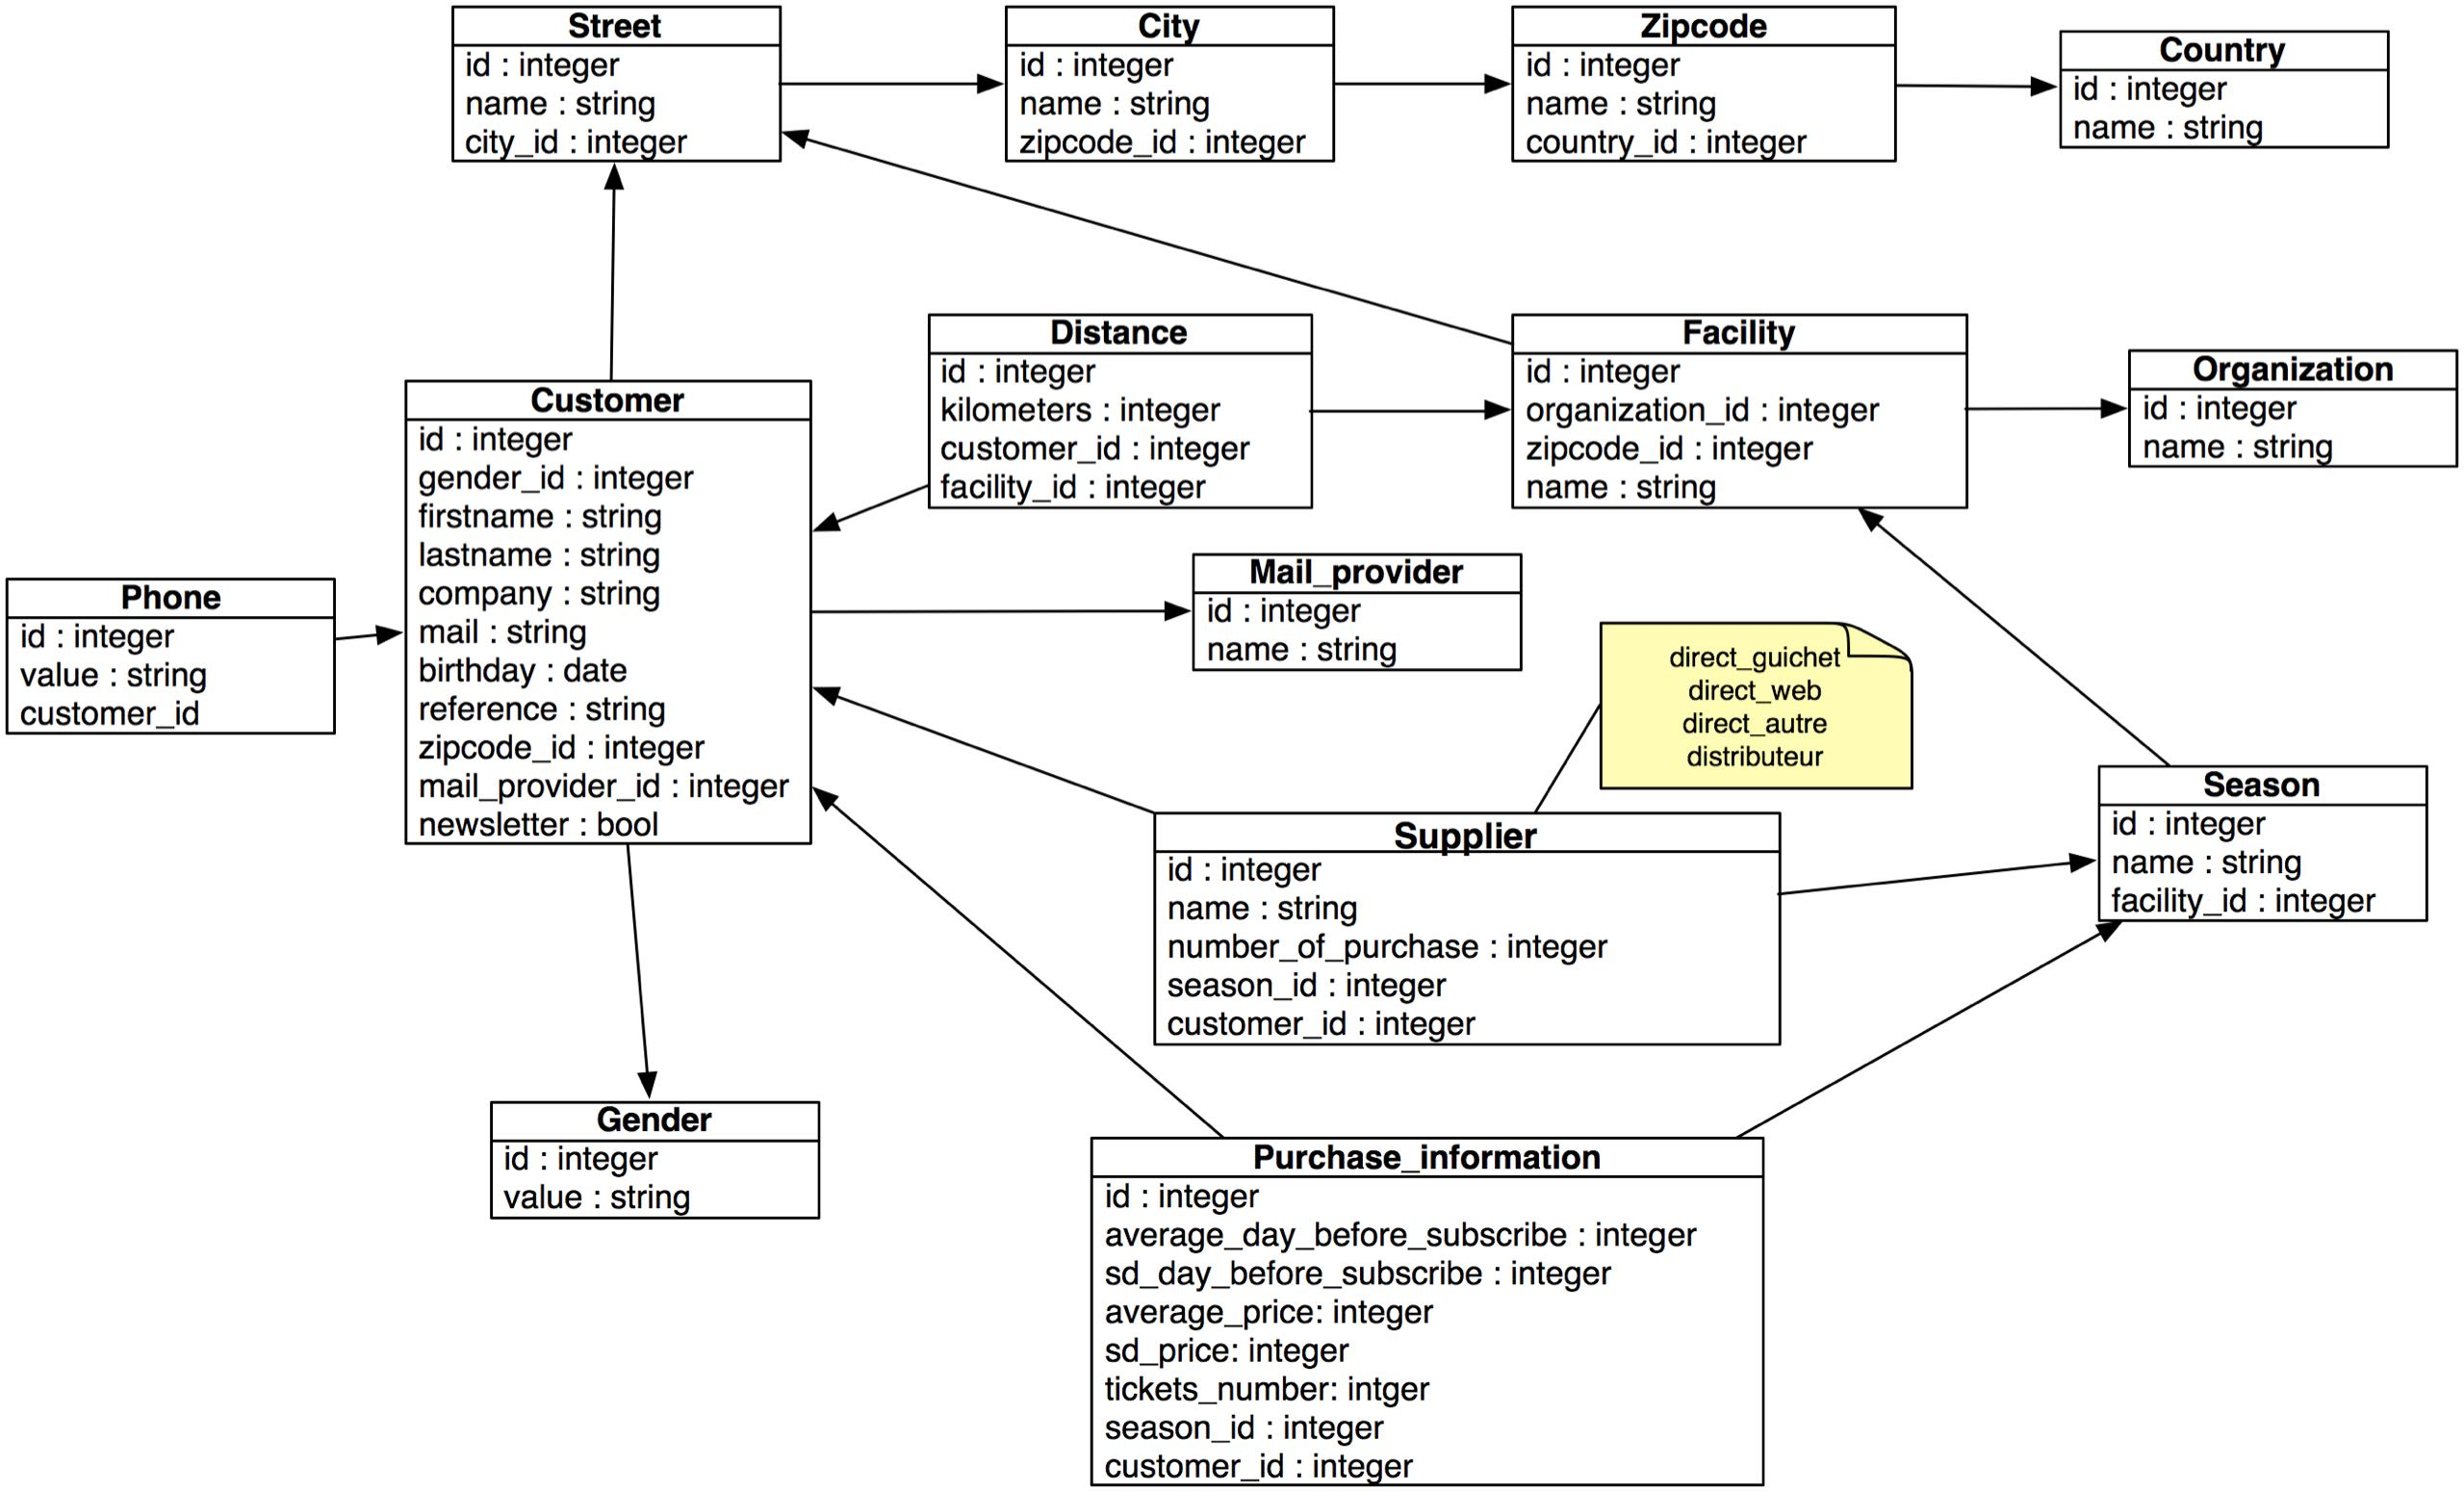
\includegraphics[scale=0.2]{images/arenapublic-1.jpg}
\captionof{figure}{Premiere architecture de la base de données ArenPublic}
\label{arenapublic-1}
\end{center}


Comme le montre l'archtecture de base de données \ref{arenapublic-1} page \pageref{arenapublic-1} des données comme des écarts types et des moyennes dans les tables Supplier et Purchase information sont calculés. Le problème est qu'il nous faut pouvoir ajouter de nouvelles données facilement en fonction de la demande du client ou du besoin des statisticiens.

Nous décidons donc d'utiliser en complément de la base de donnée SQL une base de base de données de type NoSQL \footnote{Not only SQL} qui permet de rajouter des informations "à la volée" sans modifier la structure de la base de données. 

\subsection{Implémentation téchnique}
Pour la base de données NoSQL nous voulons quelques chose de simple à mettre de oeuvre de type clé valeur. Nous utilisons donc le système de base de données décentralisé Riak qui permet de stockés des informations de type clé valeur dans un bucket.

\begin{center}
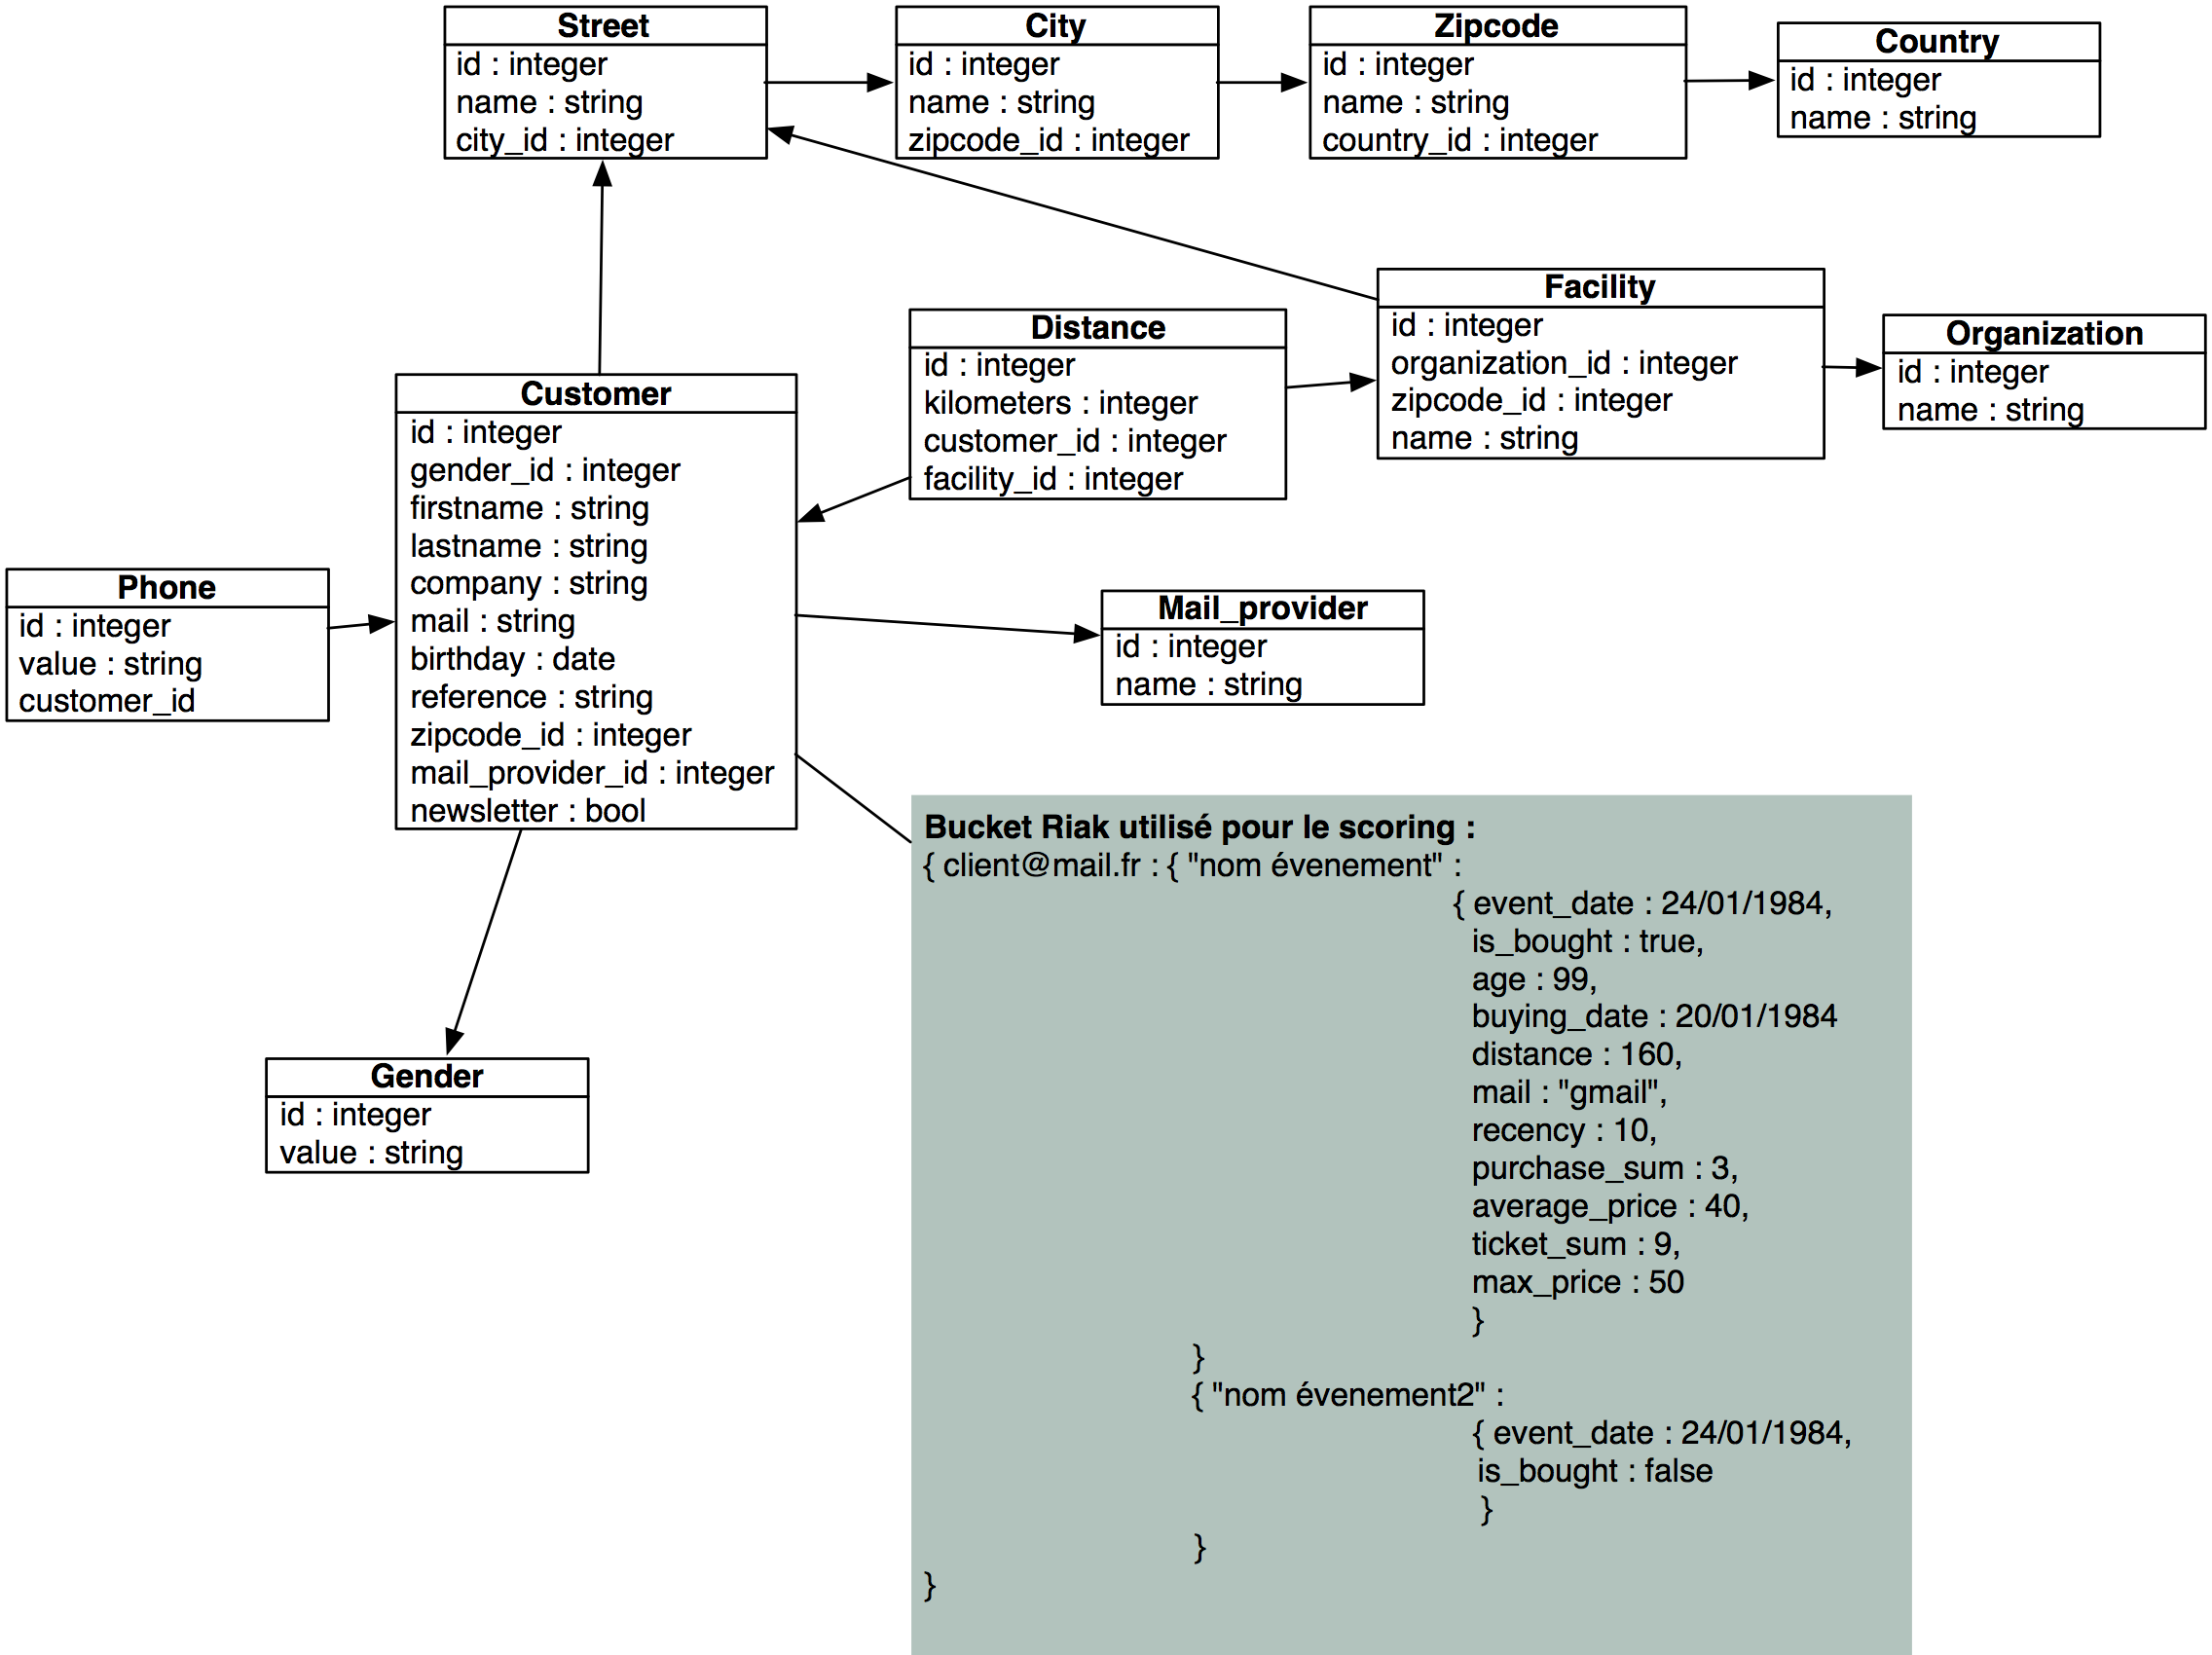
\includegraphics[scale=0.62]{images/arenapublic-2.png}
\captionof{figure}{Architecture finale de la base de données ArenaPricing}
\label{arenapublic-2}
\end{center}

Finalement nous obtenons l'architecture de base de données visible en \ref{arenapublic-2} page \pageref{arenapublic-2}.

La clé du Riak est l'adresse mail du client dans la base de données, il s'agit de la seule valeur vraiement indispensable afin de pour identifier les clients de manière unique.

\subsection{Remplissage de la base de données}

Pour remplir la base de données ArenaPublic nous pouvons utiliser deux méthodes : 
\begin{itemize}
  \item[\textbullet] Un front d'upload qui permet d'envoyer une fichier CSV avec les clients abonnées pour une saison spécifique.
  \item[\textbullet] En allant piocher diréctement dans la base de données ArenaPricing.
  \end{itemize} \
 
Pour ma part j'ai essentiellement tavailler sur l'aggregation des données depuis ArenaPricing. 
Pour faire cela j'ai utilisé le language Python car il permet de facilement gérer des dictionnaire et de nombreux modules mathématiques sont disponibles pour pour fournir au staticticiens des données aussi complète que possible. Il ne leur reste ainsi qu'à les analyser. 

\begin{center}
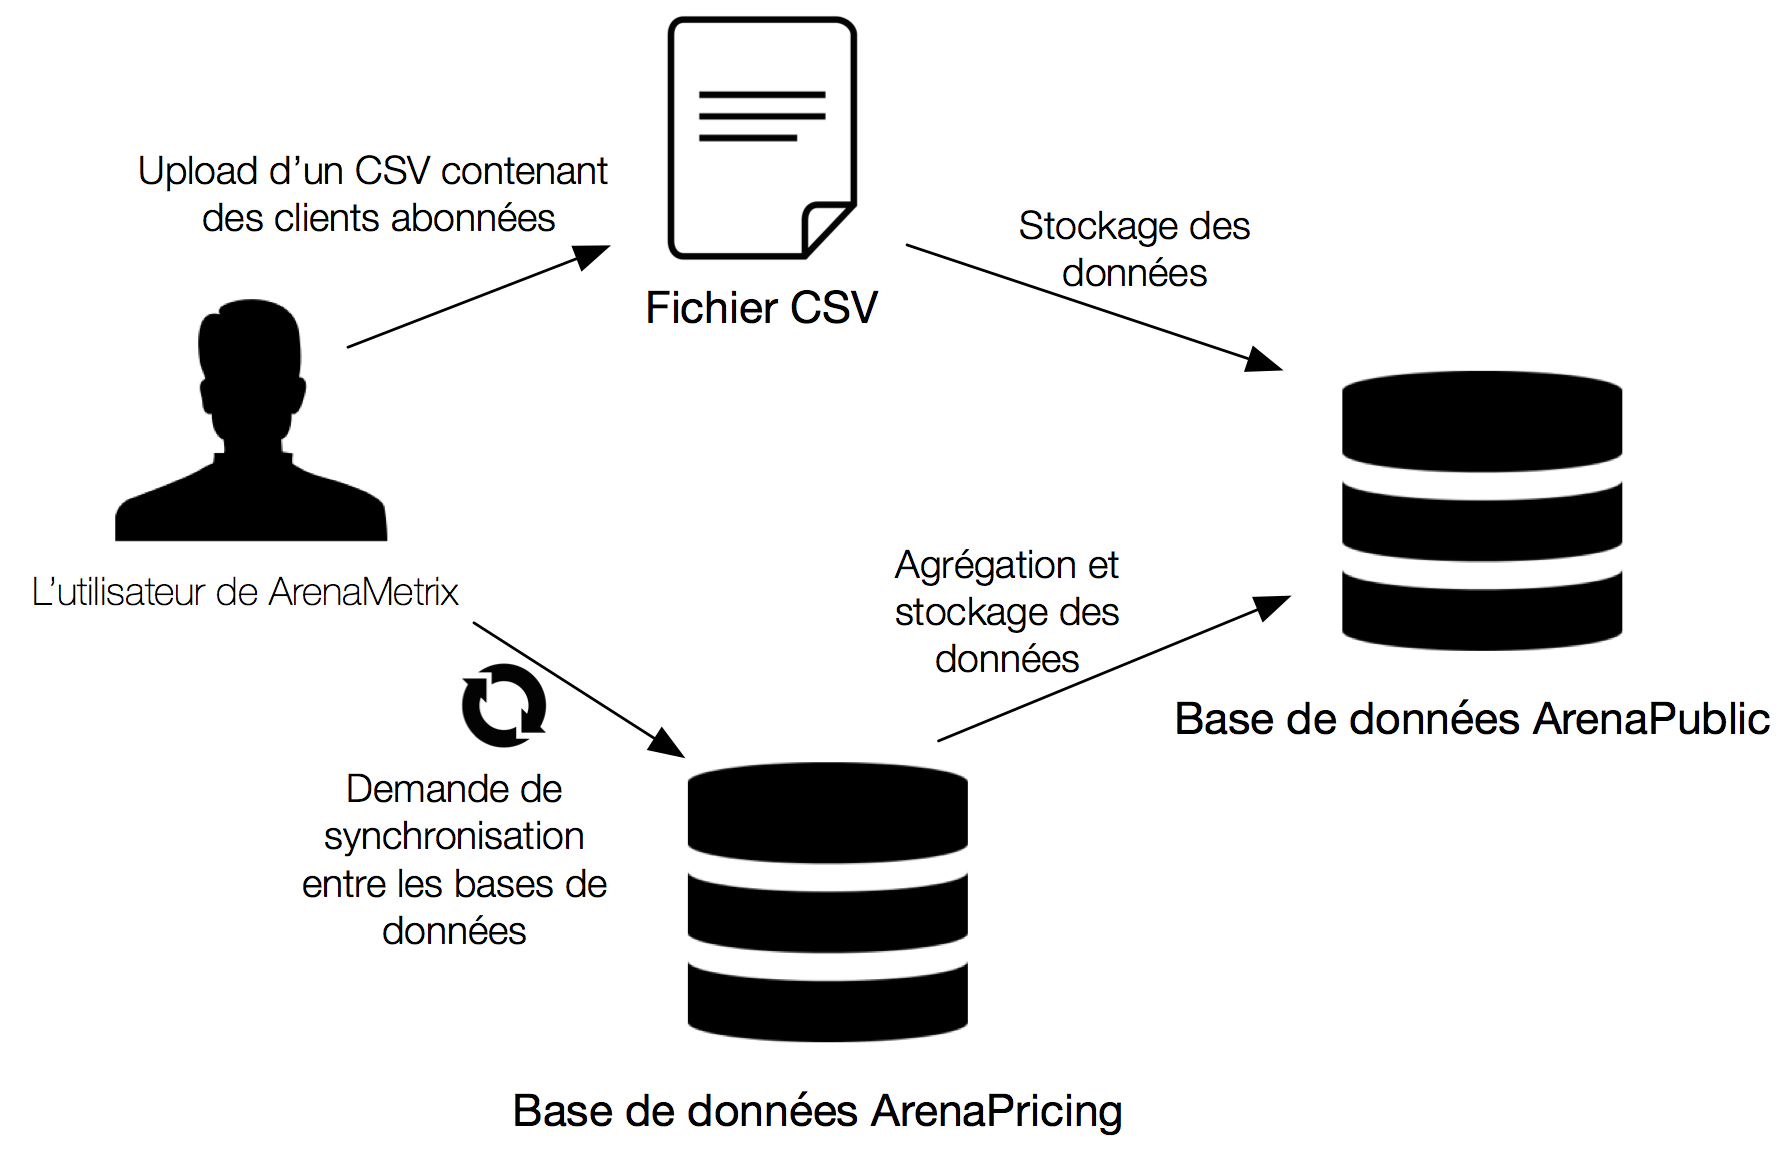
\includegraphics[scale=0.7]{images/public-to-pricing.png}
\captionof{figure}{Remplissage de la base de données ArenaPicing}
\label{public-to-pricing}
\end{center}

Comme le montre la figure \ref{public-to-pricing} page \pageref{public-to-pricing} il est possible pour l'utilisateur d'envoyer ses données au choix depuis un fichier CSV ou en synchronisant les données avec la base de données ArenaPricing. 

D'un point de vue commercial, la synchronization des données avec ArenaPricing et ainsi la réalisation d'un CRM à partir de données billéterie est uniquement disponibles pour le client ayant souscrit aux deux offres. 

Tech4Team propose ainsi deux offres de scoring différentes : 

\begin{itemize}
  \item[\textbullet] Scoring sur le réabonnement : pour les clients nous fournissants des données abonnées. 
  \item[\textbullet] Scoring sur l'achat : pour les clients ayant des données dans ArenaPricing  \end{itemize} \

\subsection{Enrichissement des données}

Lors de l'agrégation des données de ArenaPricing dans ArenaPublic en plus de faire les calcules servant aux statisticiens, j'ai enrichies les données disponibles afin d'offrir plus de possibilité au statisticiens.
\\ \\
Ajout du sexe de la personne en fonction du prénom lorsque l'information n'est pas disponible :
Pour réaliser cet enrichissement de données j'ai utilisé le module 
\href{https://github.com/ferhatelmas/sexmachine/}{SexMachine}
Ce module retourne male, female, mostly\_male, mostly\_female ou andy en fonction du prénom passe en paramètre.

\lstset{style=custompython}
\begin{lstlisting}
>> import sexmachine.detector as gender
>>> d = gender.Detector()
>>> d.get_gender(u"Bob")
u'male'
>>> d.get_gender(u"Sally")
u'female'
>>> d.get_gender(u"Pauley") # should be androgynous
u'andy'
\end{lstlisting}
\captionof{lstlisting}{Exemple d'utilisation de SexMachine}

Le problème avec le module officiel de SexMachine repertorié sur pypi est qu'il est compatible uniquement avec la version 2.7 de Python. Hors nous utilisons Python 3.X pour l'ensemble de nos logiciels et scripts Python. 

J'ai donc modifié SexMachine pour le rendre compatible avec Python 3.X. Le code source de la version modifié est disponible sur mon repository Github : \href{https://github.com/ludovicl/sexmachine}{https://github.com/ludovicl/sexmachine}.

\subsection{Calcul de la distance}

